\chapter{Theoretical Framework}

Typical galaxies contain different satellite stellar systems of between $ 10^{2} $ and $ 10^{6} $ stars which can orbit their galactic core. We call these interesting systems star clusters and they are basically divided into three main types: Open Clusters, stellar associations and \textbf{Globular Clusters}. Open clusters are stellar systems that can contain from hundreds to thousands of stars, they are formed continuously in the Galactic disk and most of them are relatively young (younger than 1 Gyr). Old open clusters are rare since their gravitational stability is very low and can be easily disrupted by gravitational shocks from passing interstellar gas clouds. It seems likely that most of the stars in the galactic disk were formed in open clusters that have dissolved since then. 

Stellar associations such as young associations of stars that can contain 10 to 100 massive stars of spectral class O and B, and are known as OB associations. These associations also contain hundreds or thousands of low- and intermediate-mass stars.

Globular clusters, the other important class of stellar systems, are much more interesting and in this thesis we study deeply their properties and characteristics. Although we agree that one may find young globular clusters in galaxies, we will focus our discussion on old globular clusters and unless we mention it explicitly, we will refer al all time to old globular clusters. 

For a proper and more general introduction of the theory behind the study of our target object $\omega$ Centauri, we first discuss in detail the mathematical and theoretical treatment of old globular clusters as a whole and then focus explicitly to this Globular Cluster. 

\section{Basics of Globular Clusters}
 
Globular clusters are very massive, bound stellar systems that can contain from thousands to millions of stars in a nearly spherical distribution spread over a volume of tens of parsecs in diameter. These stellar systems are composed of old stars and they do not contain a significant amount of gas or dust. As an example, figure 2.1 shows M15 Globular Cluster, discovered by Jean-Dominique Maraldi in 1746 while he was studying the De Chéseaux comet, the cluster shows the spherical symmetry and a higher stellar density in the center, it can also be seen that most of the cluster brightness is given by the stars and not by dust or gas.

\begin{figure}[H]
\centering
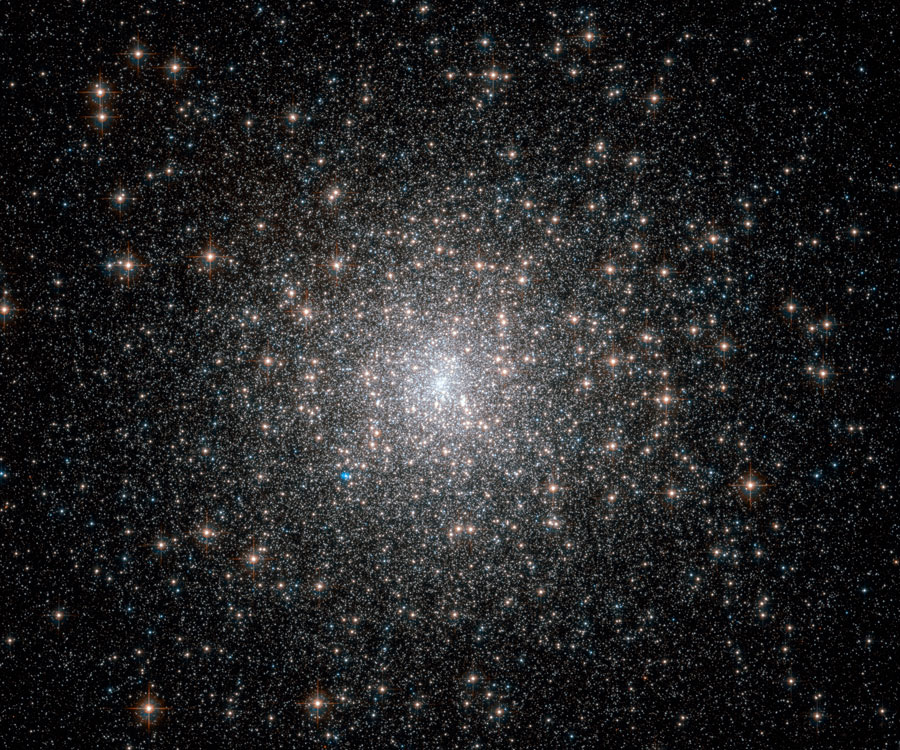
\includegraphics[width=12cm]{images/m15.jpg}
\caption[M15 Globular cluster]{Globular Cluster M15, taken by the Hubble Space Telescope with an exposition time of 900 seconds. The spherical symmetry  that is clearly seen is one of GCs' most representative properties. Image credit by NASA}
\end{figure}

These stellar structures are compact, gravitationally bound groups of hundreds of thousands to several million stars that are themselves gravitationally bound to galaxies. They have comparable ages to their associated galaxies which is an encouraging characteristic to study them as they could provide valuable information about the formation and evolution of their host galaxies.

Their star populations are uniformly old, although different stellar populations are found as we improve our measurements and observations, such as in the case of the recent study of the stellar populations in the globular clusters of the Fornax dwarf galaxy, where multiple stellar populations and nitrogen abundances have been found (Larsen \& Brodie et al. 2014). Globular clusters are devoid of gas so that pretty much no new stars form in them. The stars at the centre of a globular cluster are much more densely packed than the stars in other parts of the galaxy, providing a rather hostile scenario for the formation of habitable planets.

Globular clusters revolve about the nucleus of a galaxy on orbits of high eccentricity and high inclination to the galactic plane. About a third of globular clusters are concentrated around the galactic center (Talpur, 1997). A typical cluster has a period of revolution around the order of $ 10^{8} $ years. A cluster spends most of its time far from the center of a galaxy, and so most of them can, and have been discovered in the spaces between galaxies. 

Due to clusters moving in various orbits in the Galaxy, they are bound together with gravitational forces that are stronger than the disrupting forces exerted on it by the Galaxy or other nearby stars, and this results in an added condition for the stability of a cluster (Talpur, 1997).

The spherical shape of these systems is due to the stability that they can acquire over time. To ensure the stability of an isolated cluster, the average speed of its individual stars must not exceed the escape velocity from the cluster. If this occurred, the stars would escape into space, and the cluster would dissipate. If the stellar velocities are low enough to satisfy this condition, then the cluster is gravitationally bound, i.e. the force of gravity is strong enough to keep the member stars from escaping.

Another factor in the stability of clusters is size; the smaller and more compact the cluster, the greater its own gravitational binding force compared with the disrupting forces, and the more chance it has to survive to old ages.

Because globular clusters are highly compact systems, they are consequently very stable, and so most globular clusters will probably maintain their identity almost all of their lifetimes. But even these clusters lose some stars, especially if they have a low mass. This is because there are always some stars in the cluster that can eventually reach velocities high enough for them to leave the gravitational pull provided by the mass of the cluster.

When a star escapes, it carries with it energy, removing this energy from the cluster as a whole. This eventually results in the cluster developing a tightly bound core surrounded by a rarefied halo of stars as we can see in figure 2.2 which is a set or observations of three galactic globular clusters:

\begin{figure}[H]
\centering
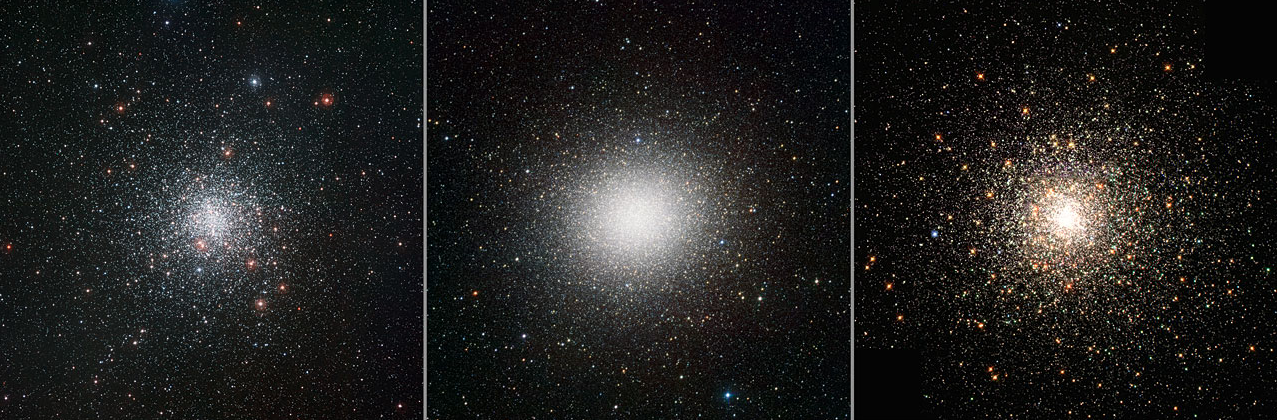
\includegraphics[width=14.5cm]{images/3_gcs.png}
\caption[ESO and Hubble images of Globular Clusters]{Globular Clusters taken by ESO and the HST. From left to right: M4 (ESO), Omega Cen (ESO) and M80 (Hubble). Images from the Hubble Space Telescope database.}
\end{figure}

In the dense core of a cluster, the stars occasionally collide, and some of the debris eventually coalesces. Predictions indicate that this dynamical evolution could lead to the development of a large Black Hole at the cluster's center. At the same time, a few stars in the outer parts of the cluster would continue to escape. The escape rate and dynamical evolution for the rich globular clusters are so slow that the clusters can easily survive for many billions of years, remaining mostly unchanged.

Observations and mass models of these structures show that the average star density in a Globular Cluster is about 0.4 stars per cubic parsec. In the dense center of the cluster, the star density can increase from 100 to 1000 stars per cubic parsec. However, even in the center of clusters, there is still plenty of space between the stars.

In order to understand how dense Globular Clusters can be, we may think of a clear example like Proxima Centauri, which is about 1.3 parsecs from Earth. Thus, if we were able to draw a sphere around the Sun with a radius of 1.3 parsecs, it would only contain 2 stars: the Sun and Proxima Centauri. But if you were to draw this same sphere in the center of the globular cluster M13, it would contain approximately 10,000 stars.

\section{Formation and evolution}

The formation of Globular Clusters is not well understood yet, and we only have crude ideas of their typical states right after they have reached the dynamical equilibrium. As it was mentioned in the introduction, two main broad types of possibilities have been considered to explain the very first processes that created these structures. 

The first scenario suggests that in the early universe the first structures that came to exist were globular clusters formed by Jeans instability. One of the main contributions to this possibility was given by Peebles \& Dicke (1968) who first pointed out that globular clusters might have formed even before the collapse of the protogalaxy, noting the fact that the baryonic Jeans mass right after decoupling is about the size of a Globular Cluster. Although their possibility is in concordance with the current scenario of galaxy formation, there are still problems of this theory, for example, it cannot explain why there are so few intergalactic globular clusters and why the properties of globular clusters are correlated with their host galaxies. As mentioned before, another problem with this theory are the observational results of Odenkirchen et al. (2003) of the tidal tails of some GCs that could not exist if these stellar systems had their own dark matter halos that would keep the stability and thus avoiding the creation of these tidal tails.

The second formation scenario suggests that Globular Clusters are secondary objects, and they could have been formed by thermal instabilities in cooling halo gas or by gravitational instabilities in giant bubbles or even by the shocked layers between two colliding clouds. 

The theory about the thermal instabilities in cooling halo gas proposed by Fall \& Rees (1985, 1988)  suggests that cold dense clouds condense out of hot and tenuous background to form as progenitors of globular clusters. This idea could be in accordance with the present observational properties of Globular Clusters like their characteristic metallicity. Yet again, this theory has proven difficulties to justify the assumed thermal behaviour of the cluster-forming gas clouds and the existence of globular clusters in very low mass galaxies (Harris \& Racine, 1979).

The idea that GCs were formed by gravitational instabilities in giant bubbles and busted by the shock of layers between two or more colliding clouds has been defended by some authors such as Murray \& Lin (1992) who have argued that self-gravitating clouds are unstable to fragmentations and spontaneous star formation so that these stellar systems must form from sub-Jeans mass clouds. In subsequent work, published in 1993 by Murray et al., it has been shown that only clouds in a limited mass range ($10^{4}M_\odot\lesssim M\lesssim 10^{6}M_\odot$) can survive both the Kelvin-Helmholtz instability of the gas and the thermal instability of the system which does not lead to bound clusters. Clouds within this critical mass range will form globular clusters if they are induced into cooling and collapse by collisions with sufficient velocity. As it can be seen, the formation of these ancient structures is in a current debate (Larson 1996) and is directly correlated with the formation of galaxies itself so they could provide answer to our ever changing modelling. 

Moving on to the evolution of these systems, we note that our current observations and modelling give us good results after the equilibrium has been reached, in this context, there must be mentioned that the mechanism that drives the system to stability is \textbf{relaxation} (explained in the next section). This process pretty much erases the cluster's memory of it's initial state so the results for gravitational stable systems can be reached using a wide range of initial conditions and they can be easily modelled.

For a typical Globular Cluster with $N=10^{5}$ stars and a radius of $r=10\:\:pc$ the relaxation time would be around $t_{relax}=10^{9}\:years$ which is much smaller than the age of the stars in the GC so that stability can (and is observed to) be easily reached. Since the relaxation time is inversely proportional to density, then evolution due to this mechanism proceeds most rapidly in the dense central regions of the clusters. Within this central region that is relaxed, the distribution function $f$ and the density distribution should be approximate to a isothermal distribution, this means that the distribution function must be approximately Maxwellian at energies well bellow the escape energy. We assume that in the outer parts of the clusters the relaxation time is long and encounters have relatively little effect.

Other important characteristic of their evolution is that they lose mass from stellar evolution: Our stellar evolution theories show us that stars usually eject mass from their surfaces near the ends of their lives, this is a well studied problem. For the mass-losing stars inside globular clusters, the ejected mass is likely to escape the cluster, either because the ejection velocity exceeds the escape speed from the cluster or because it interacts with the galactic gas when the cluster is passing through the disk, assuming this is the case. So we can conclude that the clusters lose mass as stars evolve. It must be mentioned that the evolution time scale of a typical population of stars is usually much longer than the crossing time in the cluster.

The mass lost by a cluster due to stellar evolution depends on the initial mass function which specifies the distribution of masses of stars just after they have formed and the initial-final mass function. 

Now, when we talk about the evolution of Globular Clusters, we must see how the mass distribution evolves over time mainly because this will help us to better understand their formation. The evolution of the mass distribution in an isolated cluster such as a GC that is far enough from the disk to have few important encounters and collisions, can be modelled using the simple but powerful Plummer model that we shall introduce in the following section as shown in figure 2.3.

\begin{figure}[H]
\centering
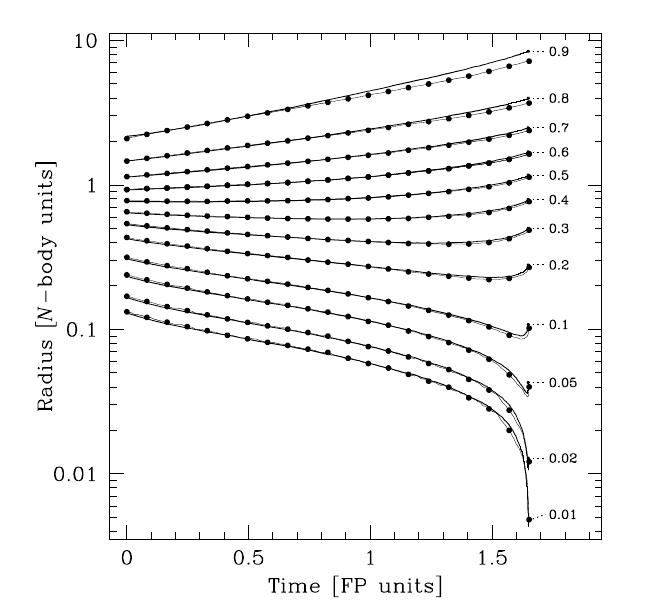
\includegraphics[width=10cm]{images/core_collapse.png}
\caption[Evolution of an ergodic Plummer model over time]{Evolution of an ergodic Plummer model over time, according to an orbit-averaged Monte-Carlo solution of the Fokker Planck equation with $3\times10^{5}$ superstars (heavy solid lines) and an N-body simulation with $65536$ superstars (dots, connected by solid lines). From Freigat, Rasio, \& Baumgardt (2006)}
\end{figure}

As we can see above, the outer half of the cluster expands, mainly due to the gradual growth of the halo as stars in the core diffuse towards the escape energy, but the most important feature of this figure, is that we can see that the center contracts or gets smaller, this process is known as \textbf{core collapse} and it leads to a dramatic growth in the central density that may indicate the existence of an apparent singularity in the central density such as a black hole.

Takahashi (1995) found a more accurate calculation of core collapse in a spherical cluster (without binaries) starting from a Plummer model. His calculations allow greater dynamic range than Monte Carlo or N-body methods. His results show that as the cluster evolves, the core radius shrinks  and the central density grows, as seen in the above figure. Outside the core, the density profile approaches a power law of the form $\rho\varpropto r^{-2.23}$.

Another interesting result regarding Takahashi's method based on the direct solutions of the orbit-averaged Fokker Planck equations (partial differential equations that describe the time evolution of the probability density function of the velocity of a particle under the influence of dragging and random forces) is the behaviour of the anisotropy parameter $\beta=1-\overline{v_{\theta}^{2}}/\overline{v_{r}^{2}}$ as we can see in figure 2.4.

\begin{figure}[H]
\centering
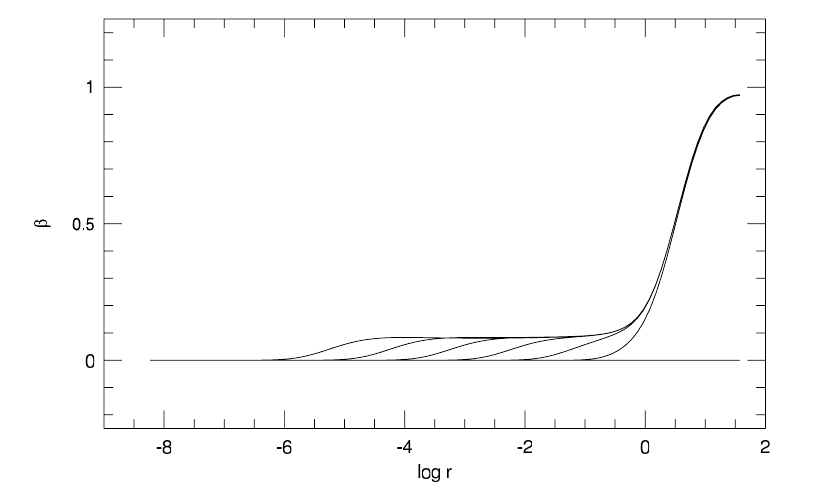
\includegraphics[width=12cm]{images/anisotropy_core_collapse.png}
\caption[Evolution of the velocity anisotropy parameter]{The evolution of the velocity anisotropy parameter for an orbit-averaged Fokker Planck calculation of core collapse. From Takahashi (1995)}
\end{figure}

At large radii, the anisotropy parameter (that indicates the tendency of the system to have or not preferred directions) tends to unity ($\beta\simeq1$), and that indicates that the orbits are nearly radial, at the smalest radii, inside the shrinking core, we have $\beta\simeq0$, which indicates that the velocity distribution is isotropic. We note that in the radius range in which the density profile in the top panel is a power law, there is a constant small radial anisotropy of $\beta\simeq0.08$ or  $\overline{v_{\theta}^{2}}/\overline{v_{r}^{2}}\simeq0.92$. We will discuss the details of these parameters in the next section.

Now, regarding the late interactions and accretion processes that could affect the evolution of GCs, we note that although our Galaxy has evidently not experienced any further major accretion events capable of disrupting the disk, it is possible that minor accretion events affecting only the halo and not the disk have continued to occur as suggested by Navarro, Frenk, \& White 1994, but their net effect on the GC's dynamics and stability is the context of cosmology is very low.

The evolution process for these systems is so long that it fits entirely in the context of Cosmology. Most of the clusters whose masses are larger than $10^{5}M\odot$ have lifetimes longer than the Hubble time.

\section{Observational Properties}

Galactic Globular Clusters are relatively easy to observe because they are close to us in the galactic context and their big size makes them bright objects, for this reason, they have been observed even since the 17th century. The first globular cluster discovered, but then taken for a nebula, was M22 in Sagittarius, which was probably discovered by Abraham Ihle in 1665. This discovery was followed by that of southern $\omega$ Centauri (NGC5139) by Edmond Halley in 1677, which is the largest known globular cluster in our galaxy and also a former galactic-nucleus candidate. This ``nebula" had been known but classified as star since ancient times. The next discovery was made by Gottfried Kirch in 1702 M5 in Serpens Caput, and then M13 in Hercules, again by Halley, in 1714. Charles Messier was the first to resolve one globular cluster, M4, but still referred to the other 28 of these objects in his catalog as ``round nebulae". 

By 2010, there were about 157 confirmed Globular Clusters in the Milky Way (updated Harris catalogue based on the original paper Harris, W.E. 1996) and the number is growing since we are improving our techniques to find globular clusters that may be passing through the disk and thus are difficult to observe.

Regarding their mass content, as mentioned by Roueff et al. 1997, there is  widespread belief that globular clusters cannot contain large amounts of dark matter, because of the observational results wouldn't match the  Virial Theorem. This theorem relates the velocity dispersion $ \sigma $ at the center of the cluster to the total mass $M_{t}$ and to the half-mass radius $r_{h}$ of the system. For a one component globular cluster (no dark matter), that relation may be expresed as (Spitzer 1987):

\begin{equation}
\left\langle \sigma^{2}\right\rangle \approx0.4\frac{GM_{t}}{r_{h}}
\end{equation}

The observed central velocity dispersion in the clusters do not seem to show the presence of a non-baryonic component but although the use of the virial theorem to find the mass of a Globular Cluster could be a first approximation, it lacks of precision that could be acquired using more elaborated procedures involving the presence of dark matter. The mass modelling of these objects is still being debated since the existence of dark matter in the clusters is a mystery and further work (including the effects of the stellar populations) needs to be done to clarify the scenario and give us a stronger idea on how these objects and galaxies form. 

Regarding the stellar populations, we note that these structures were once thought to consist of a single population of stars that all formed together. However, research has since shown that many of the Milky Way's globular clusters have far more complex formation histories and are made up of at least two distinct populations of stars (Larse et al. 2014). A way of analysing the stellar populations in GCs is to use Colour-Magnitude diagrams. These diagrams plot the apparent magnitudes of the stars in a cluster against their colour indices. Globular Clusters nearly all have very similar colour-magnitude diagrams.

This diagram for a typical globular cluster looks very different than that of an open cluster. There are no Main Sequence stars of types OBAF, but there are many red giants. The brightest stars in a globular cluster are those at the tip of the red giant branch in the color-magnitude diagram, which explains the red appearance of the bright stars in color images of the clusters. You can also see stars populating the horizontal branch (and also why it is called the horizontal branch), the asymptotic giant branch, and even some stars that have colors and magnitudes of F stars, but far fewer than the G stars just below and to the right of them on the Main Sequence. In order to see the characteristics of these diagrams, figures 2.5 and 2.6 show the difference between the color-magnitude diagram of a typical globular cluster (M55 in this case) and that of generic stars outside GCs.

\begin{figure}[H]
  \centering
  \begin{minipage}[b]{0.44\textwidth}
    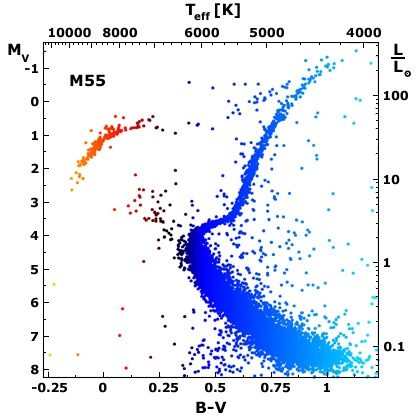
\includegraphics[width=\textwidth]{images/m55_diagram.jpg}
    \caption[Color Magnitude diagram of M55]{Color Magnitude diagram of M55 Globular Cluster. Over time, higher mass stars have evolved off the main sequence into red, then blue giants and beyond. The exact position of the sharp turn-off from the main sequence to the red giant branch measures the cluster's age. Image by NASA.}
  \end{minipage}
  \hfill
  \begin{minipage}[b]{0.55\textwidth}
    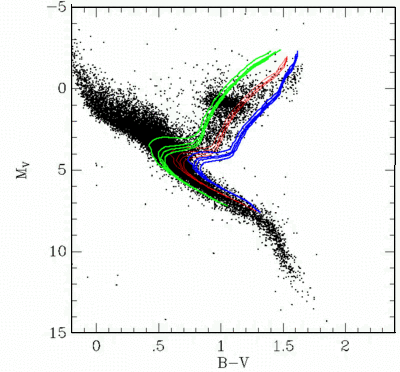
\includegraphics[width=\textwidth]{images/color-magnitude.png}
    \caption[HR Diagram for Stars]{Colour magnitude diagram for nearby stars, with 3 isochrones of differing age overlaid (and four different metallicities each). The oldest stars in the disk have ages of about 10 Gyr. Source preprint. Jimenez, Flynn \& Kotoneva, 1998.}
  \end{minipage}
\end{figure}
 
Of the GC's stellar populations, around half the stars are a single generation of normal stars that were thought to form first, and the other half form a second generation of stars, which are polluted with different chemical elements. In particular, the polluted stars contain up to $50 \sim 100$ times more nitrogen than the first generation of stars (Larse et al. 2014).

The proportion of polluted stars found in the Milky Way's globular clusters is much higher than astronomers expected, suggesting that a large chunk of the first-generation star population is missing. A leading explanation for this is that the clusters once contained many more stars, but a large fraction of the first-generation stars were ejected from the cluster at some time in its past (Charbonnel et al. 2014).

In the past, we didn't know whether globular clusters in smaller galaxies had multiple stellar generations or not, but recent observations show clearly that they do (Larse et al. 2014). This finding means that a leading theory on how these mixed-generation globular clusters formed cannot be correct, and astronomers will have to think once more about how these mysterious objects in the Milky Way and further afield came to exist.

For the most part, GCs have low metallicities since they have predominantly only one generation of stars. As shown in figure 2.7, the metallicity (Fe/H) of globular clusters is very low compared to the one of stars in the solar neighbourhood. The metallicity of a globular cluster can be inferred using stellar spectra by comparing the amount of iron  to the amount of hydrogen or by adjusting isochrones to the color magnitude diagrams of the clusters. Detailed studies using both techniques have shown us that although metal rich stars in the cluster are uncommon, they are present in the clusters and they could provide evidence on what types of interactions with the interstellar medium or galactic disk have taken place or what kind of evolution processes we don't know about these stellar systems.

\begin{figure}[H]
\centering
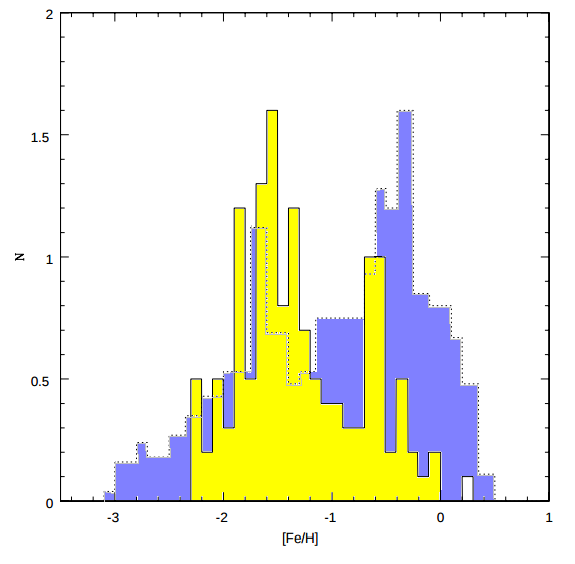
\includegraphics[width=8cm]{images/metal.png}
\caption[Metallicity of GCs compared to stars in the solar neighbourhood]{Metallicity distribution functions for comparison: The full line are the data corresponding to the globular clusters in our Galaxy, taken from Harris (1999); dashed line are the data corresponding to the stars in the solar neighbourhood, taken from Carney et al. (1990). This plot was made by Casuso \& Beckman (1991)}
\end{figure}

One important development regarding GCs is some debated observational evidence that dense, massive star clusters are currently forming in certain environments such as giant molecular clouds (Harris \& Pudritz 1993). It has been suggested that these objects are young globular clusters. This idea is not universally accepted, both because current observations are not definitive and possibly because of the notion of globular clusters as ancient objects. However, if globular clusters are forming at the present epoch, we will have the opportunity to study the formation process directly (Portegies 2010). It seems inevitable that this will greatly enhance our understanding of how and why globular clusters form, as well as deepening our knowledge of the galaxy formation process to which globular cluster formation is intimately related.

Some other observational results of GCs in other galaxies just broadens the current scenario of formation and evolution, for example, in November, 2014 Tim Stephens from the University of California studied images taken by the HST of four globular clusters located in the small galaxy Fornax to study their properties and compare them with GCs in the Milky Way. What these observations show is that the GCs in the dwarf galaxy Fornax are very similar to our GCs and so they must have formed in a similar way, however, these findings don't fit with the leading theories that have been developed to explain how globular clusters form in such a dwarf galaxy. Figures 2.8 and 2.9 show the HST images of two of the studied globular clusters by Tim Stephens.   

\begin{figure}[H]
  \centering
  \begin{minipage}[b]{0.49\textwidth}
    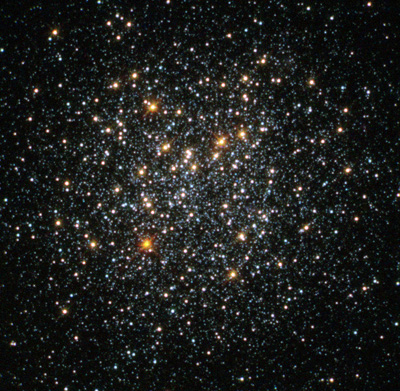
\includegraphics[width=\textwidth]{images/fornax-2-400.jpg}
    \caption[Hubble image of Fornax-2 Globular Cluster]{Image of Fornax-2 Globular Cluster taken by the Hubble Space Telescope. From University of California newscenter.}
  \end{minipage}
  \hfill
  \begin{minipage}[b]{0.49\textwidth}
    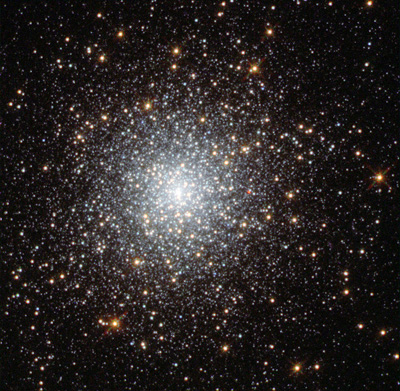
\includegraphics[width=\textwidth]{images/fornax-3-400.jpg}
    \caption[Hubble Space Telescope image of Fornax-3 Globular Cluster]{Hubble Space Telescope image of Fornax-3 Globular Cluster. From University of California newscenter.}
  \end{minipage}
\end{figure}

As mentioned before, the proportion of nitrogen-rich stars in the Milky Way's GCs seems to be higher than astronomers expected. This suggests that a large chunk of the first-generation star population is missing to account for the high metallicity of the observed stars. One fair explanation that astronomers have adopted is that clusters once contained many more stars but a large fraction of the first-generation stars were ejected from the cluster at some time in its past. In our galaxy, these stars could go to the halo.

Now, the observations of the Globular Cluster in Fornax contradict this hypothesis since they have found that the proportion of second-generation stars is quite similar to that of the GCs in the Milky Way, but unlike our galaxy, Fornax doesn't have enough old stars to account for the huge number that would have been vanished from the clusters, and we should be able to see them but we don't (Lars et al. 2014).

These types of findings mean that a leading theory on how these mixed-generation globular clusters formed cannot be correct and astronomers will have to reconsider how these mysterious objects, in the Milky Way and further afield, came to exist.

Another important observational property of the globular clusters is that it is possible to use various techniques such as fitting isochrones to the color magnitude diagrams,  analysing the horizontal branch or binning the stellar luminosity function in order to determine the age of the clusters. Jimenez, 1998 found that the oldest galactic GCs have an age of $13.5 \pm 2$ Gyr which is in agreement with  Krauss \& Chaboyer (2003) results. That the GCs are so old is yet another valuable observational result that shows us how important it is to understand these objects in the context of galaxy formation and evolution. 

Now, for the spatial distribution, we have that radial velocity measurements have revealed that most Globular Clusters are moving in highly eccentric elliptical orbits that take them far outside the Milky Way; they form a halo of roughly spherical shape which is highly concentrated to the Galactic Center, but reaches out to a distance of several thousands of parsecs, much more than the dimension of the Galaxy's disk. They are located at distances of thousands of parsecs from the bulge and most of them are separated from the galactic disk so they don't have strong interactions with the gas. Figure 2.10 shows the spatial distribution of some of the galactic globular clusters within a radius of 15330 parsecs relative to the center of the galaxy.       

\begin{figure}[H]
\centering
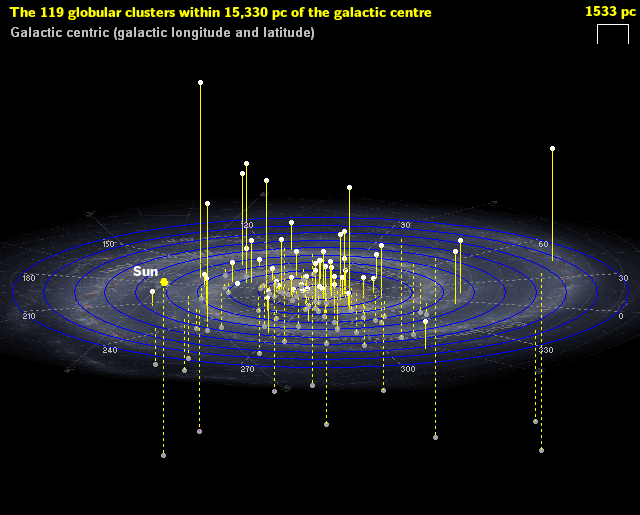
\includegraphics[width=10cm]{images/Globulars4.png}
\caption[Spatial distribution of globular clusters in the Milky Way]{Spatial distribution of globular clusters in the Milky Way that are within a radius of 15330 parsecs. The figure shows the position of the Sun in the plane of the Galaxy. Data from William E. Harris, McMaster University. 3D image by Larry McNish \cite{18}}
\end{figure}

As they don't participate in the Galaxy's disk rotation, they can have high relative velocities of several 100 km/s with respect to our Solar System; this is what shows up in the radial velocity measurements. We could picture their orbits around the galaxy as shown in figure 2.11.

\begin{figure}[H]
\centering
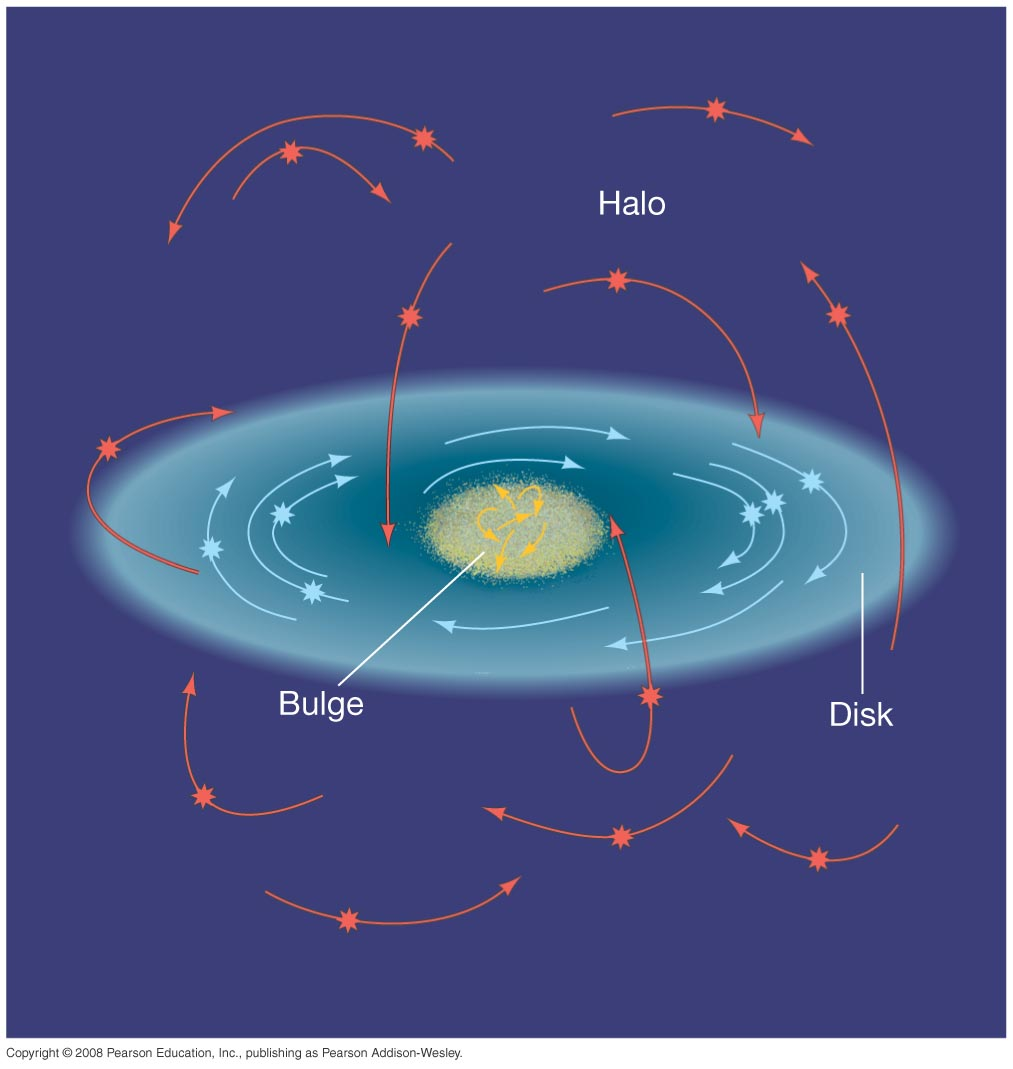
\includegraphics[width=10cm]{images/orbits_gcs.jpg}
\caption[Illustration of the orbits of Globular Clusters around a spiral galaxy]{Illustration of the orbits of some Globular Cluster in a spiral galaxy like the Milky Way. Picture from the Oregon University webpage \cite{22}}
\end{figure}

One problem that has been debated (Jouse \& Wiegandt 1977) is the size of the eccentricities of their orbits. Since the encounters between clusters are too rare to produce any internal relaxation, then the present distribution of cluster orbits should be close to that prevailing at their formation, except possibly in the cery central regions and or course the disk, where dynamical friction could change the orbits (Tremaine et al. 1975, Keenan 1978).

Now, when we talk about the observational properties of GCs, we must mention photometric and spectroscopic observations of individual stars in the Clusters, which can be achieved since the clusters are not too far away for our observations to be imprecise. In the context of dynamics, recursive photometric observations of cluster members can in principle give us information about their proper motion in the plane of sight, in addition to radial velocities, we could reconstruct their 3D velocity profile and the overall rotation of the clusters. 

Individual spectroscopic observations, on the other hand, can be very useful for reconstructing the velocity dispersion profile of the cluster. This can be made using the Doppler shift of the spectral lines in the spectra, by cross correlating the observed spectra with a rest frame spectrum and measuring the projected radial velocity of the stars, result of the cross correlation. The mathematical treatment that has to be done to infer the velocity dispersion profile and obtaining information about the potential well is well described in the next section.

For elliptical galaxies, and thus globular clusters, the \textbf{surface brightness} usually follows a Sersic profile of the form: 

\begin{equation}
I(R)=I_{e}e^{-b_{n}\left[\left(\frac{R}{R_{e}}\right)^{1/n}-1\right]}
\end{equation}

where $I_{e}$ is the intensity at the effective radius $R_{e}$ that encloses half of the total light from the model (Caon et al. 1993). For the special case of $n=4$ we have the De Vaucouleurs profile:

\begin{equation}
I(R)=I_{e}e^{-7.669\left[\left(\frac{R}{R_{e}}\right)^{1/4}-1\right]}
\end{equation}

That we shall use to find the effective radius in our modelling using the observational data.

\section{$\omega$ Centauri}

We focus on the study of $\omega$ Centauri not only because it has special characteristics compared to the other galactic GC's, but because there is a large amount of observational data available that allows us to do a proper mass modelling and because we could use our results to argue about many of the theories that surround this controversial but magnificent stellar system. 

$\omega$ Centauri (or NGC5139 in the new general catalogue) is a very interesting target for many photometric and spectroscopic investigations because it has special characteristics such as being the largest and most massive of the known globular clusters in the Milky Way and because it is one of the most flattened (Meylan 1987).

It is a very large object  with an angular diameter of around 50 arcmin, compared to the moon that can deviate from 29.94 arcmin in the furthest distance from earth to about 33.66 from the nearest distance to it. It has a tidal radius of 45 arcmin (Trager, King \& Djorgovski, 1995) and it is located at a distance of around 4,808.39 parsecs given a distance modulus of 13.41 (Watkins et al. 2013 and Bellazii et al. 2004).

The cluster contains millions of stars and it has different mass estimations as shown in table 2.1

\begin{table}[H]
\begin{center}
\begin{tabular}{| c | c| }
    \hline
    \textbf{Article} & \textbf{Mass} ($M_{\odot}$) \\ \hline
    Mandushev et al. 1991 & $2.4 \times 10^{6}$  \\ \hline
    Pryor \& Meylan & $3.98 \times 10^{6}$  \\ \hline
    Meylan et al. 1995 & $5.1 \times 10^{6}$  \\ \hline
    Majewski et al. 2000 & $5.1 \times 10^{6}$  \\ \hline
    Van de Ven et al. 2006 & $2.5 \times 10^{6}$  \\ \hline
    Cassini et al. 2009 & $3.0 \times 10^{6}$  \\ \hline
    Valcarce \& Catelan, 2011 & $3.0 \times 10^{6}$  \\ \hline
    Jalali et al. 2011 & $2.5 \times 10^{6}$  \\
    \hline
  \end{tabular} 
\caption[Reported mass of Omega Centauri]{Reported values of $\omega$ Centauri's dynamical mass by different authors in chronological order}
\end{center}
\end{table}

The mass-to-light ratio of the cluster is $\Gamma \thickapprox 2.5$ (Van de Ven 2006) and it is one of few globular clusters that can be seen to the naked eye because it has an apparent magnitude of 5.33 and because it is so big (although it would look like a star) and even with a small telescope the stellar distribution can be seen. Figure 2.12 shows a composite image of the cluster with a very high resolution where it can be seen that the cluster has millions of stars spread over a nearly spherical distribution.

\begin{figure}[H]
\centering
\includegraphics[width=10cm]{images/Omega_Centauri.jpg}
\caption[Omega Centauri image]{Composite image of $\omega$ Centauri captured with the WFI camera from ESO's La Silla Observatory. The image shows only the central part of the cluster. North is up, East is to the left. This colour image is a composite of B, V and I filtered images. Note that because WFI is equipped with a mosaic detector, there are two small gaps in the image which were filled with lower quality data from the Digitized Sky Survey. Credit by ESO}
\end{figure}

$\omega$ Centauri is located in the Centaurus constellation, which is well seen in the south and partially seen in the North. This constellation is 9$^{th}$ in size position in constellations, and contains the star $\alpha$ centauri which is the third brightest star in the sky only outshone by Sirius and Canopus. It also contains Proxima Centauri which is the closest star from our sun. 

The cluster presents an overall rotational movement as shown in figure 2.13

\begin{figure}[H]
\centering
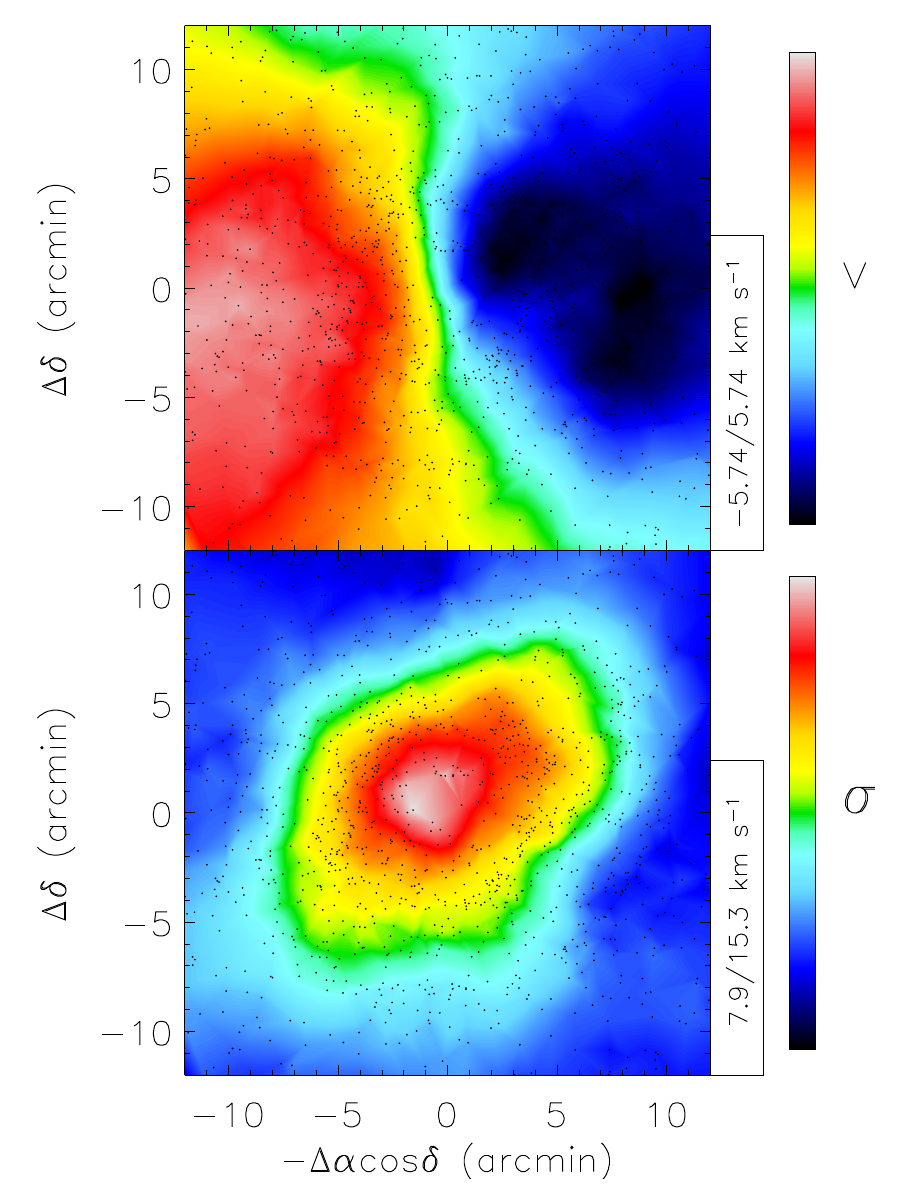
\includegraphics[width=8cm]{images/rotation_omega.png}
\caption[Omega Centauri kinematics]{This figures show the Kinematics of $\omega$ Centauri, based on adaptive smoothing of the individual measurements. a) Mean radial velocity field after subtraction of the systemic velocity. b) Radial velocity dispersion. The dots indicate the positions of the individual measurements. Reijns et al. 2005.
}
\end{figure}

The central velocity dispersion in the cluster, as shown in figure 2.13 is around $22 \pm 4km/s$ (Meylan et a. 1995) which is a direct consequence of the high mass of the system. But, besides the impressive high mass and size of the cluster, what makes it special from other galactic globular clusters?. There are three special characteristics of the cluster that make it a worth studying object with a high potential scientific value.

One is that the cluster has shown in recent studies the presence of multiple stellar populations (Bedin et al. 2004, Sollima et al. 2005). As mentioned by Bedin et al. 2004, the most evident anomaly of this cluster in comparison with the others is the large spread in metallicity seen both in spectroscopic (Norris \& Da Costa 1995) and photometric (Hilker \& Richtler 2000; Lee et al. 1999; Pancino et al. 2000) investigations. For example and most recently, Pancino et al. (2000) confirmed the existence of a very metal rich population in $\omega$ Centauri whose red giant branch (RBG) is well separated from the bulk of the RGB stars. Figure 2.14 shows a color-magnitude diagram of the cluster with a very thick main sequence, a second region in the turn off region and the metal rich population confirmed by Pancino in the vicinity of the red giant branch.

\begin{figure}[H]
\centering
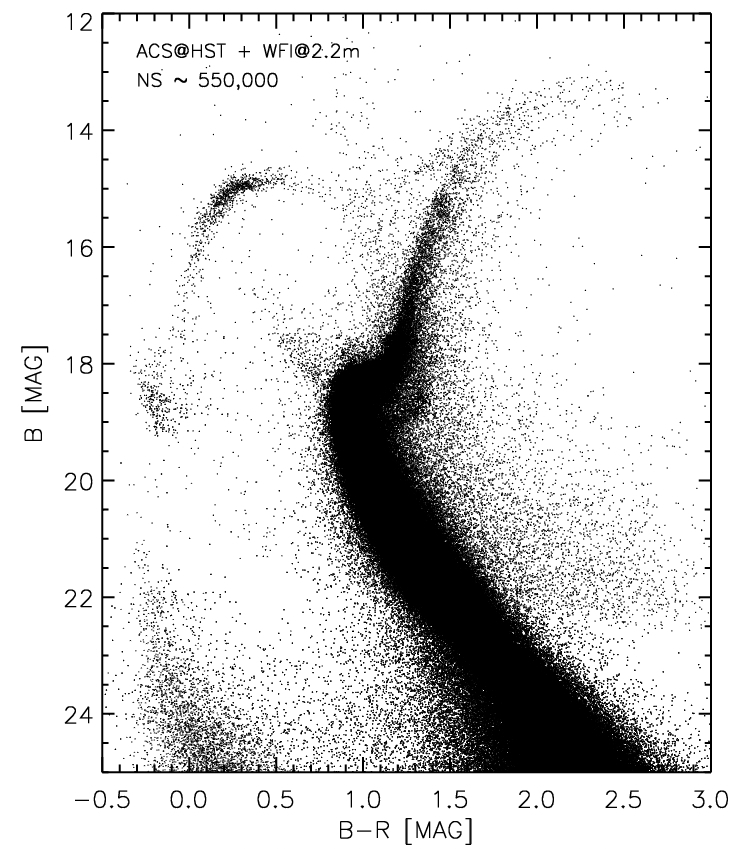
\includegraphics[width=10cm]{images/ngc5139_2.jpg}
\caption[Color magnitude diagram of Omega Centauri]{Color magnitude diagram of $\omega$ Centauri in the B and R bands with the photometric data from the Hubble Space Telescope and WFI Telescope of ESO. Photometry by Castelini et al. 2007 \& Calamida et al. 2008}
\end{figure}

Another special characteristic is that the cluster may have an intermediate mass black hole in its center with a mass of $4.0^{+0.75}_{-1.0} \times 10^{4} M_{\odot}$ (Noyola et al. 2008) that could be responsible for the increase of the central velocity dispersion in the innermost region of the cluster which is around $22 \pm 4km/s$ (Meylan et al. 2009). The theory is so attractive and likely that there have been several efforts to find the black hole in the cluster, as an example, Anderson \& Van der Marel, 2009 used a high quality proper-motion catalog in the inner region to study the presence of the IMBH but they weren't able to confirm Noyola's results. The theory of the IMBH in $\omega$ Centauri is still debated and will be subject of study for many researchers in the world because understanding the nature of intermediate mass black holes could be a hint to the understanding of the formation of supermasive black holes like those present in the center of galaxies.

Finally, one of the most exciting characteristics of $\omega$ Centauri is that it has the features of the nucleus of a former dwarf galaxy that was captured by the Milky Way. This theory suggests that the dwarf galaxy could have lost its gas and dust with the interactions with the galactic disk and could have been left with the naked core as a remnant (Hilker \& Richtler 2000). One of the consequences of this scenario if it was true is that the naked core of the dwarf galaxy could still have some dark matter inside it because dwarf galaxies are well known to have a large dark matter halo that cannot be completely stripped away with the gravitational interactions with the host galaxy. This theory has been formulated not only because the cluster is exceptionally massive but also because of its complex star formation history and the unusual high metallicities in many of the cluster members.

\section{Mass models and Dynamics}

In order to get into the physical discussions about the equilibrium and modelling of globular clusters, we need to understand first the basics of potential theory, and more specifically the potential theory of spherical systems. The next step is to discuss the physical conditions of equilibrium of these models so that the mass modelling can be made. The last but most important part is to discuss the criteria regarding the mathematical treatment of the dynamics of these systems in the context of the collisionless Boltzmann equation and the approximations to the solutions of the Jeans equations that will be used for the fitting of the observational data to do the final modelling.

\subsection{Potential Theory of Spherical Systems}

Our discussions about Potential Theory for large stellar systems will be studied using the simplifications given by the spherical symmetry of globular clusters. We first introduce some of the most important theorems for calculating the gravitational potential of a spherically symmetric distribution of matter provided by Newton, these theorems are physically related to Gauss theorem and may be proved using simple geometric assumptions or using a more precise results from vectorial calculus. More detailed procedures can be found in Binney \& Tremaine ``Galactic Dynamics" 2$^{nd}$ Edition.

\textbf{Newton's first theorem} states that a body that is inside an uniform spherical shell of matter experiences no net gravitational force from that shell. 

\textbf{Newton's second theorem} states that the gravitational force on a body that lies outside a spherical shell of matter is the same as it would feel if all the shell's matter were concentrated into a point at its center. 

It follows from Newton's theorems that the gravitational force of a spherical density distribution $\rho(r')$ on a unit mass at radius $r$ is entirely determined by the mass interior to $r$ is given by

\begin{equation}
\textbf{F}(r)=-\frac{GM(r)}{r^{2}}\hat{\textbf{e}}_{r}
\end{equation}

Where the mass as a function of the radius is

\begin{equation}
M(r)=4\pi\int_{0}^{r}dr'r'^{2}\rho(r')
\end{equation}

We can consider that the total gravitational potential of the spherical system is the sum of the potentials given by spherical shells of a differential mass $dM(r)=4\pi\rho(r)r^{2}dr$. This way, we may calculate the gravitational potential at $\textbf{r}$ generated by a spherically symmetric density distribution $\rho(\textbf{r}')$ by adding the contributions to the potential produced by shells with $r'<r$, and with $r'>r$. Thus we obtain

\begin{equation}
	\begin{aligned}	
	\Phi(r) &= -\frac{G}{r}\int_{0}^{r}dM(r')-G\int_{r}^{\infty}\frac{dM(r')} {r'}\\      &= -4\pi G\left[\frac{1}{r}\int_{0}^{r}dr'r'^{2}\rho(r')+\int_{r}^{\infty}dr'r'\rho(r')\right]
	\end{aligned}
\end{equation} 

We note an important property of a spherical matter distribution regarding its circular speed $v_{c}(r)$, defined to be the speed of a particle of negligible mass in a circular orbit at radius $r$. We may evaluate $v_{c}$ by equating the gravitational attraction $|\textbf{F}|$  to the centripetal acceleration ${v_{2}}^{2}/r$:

\begin{equation}
v_{c}^{2}=r|\textbf{F}|=r\frac{d\Phi}{dr}=\frac{GM(r)}{r}
\end{equation}

We may also note that the \textbf{escape speed} $v_{e}$ in terms of the gravitational potential is

\begin{equation}
v_{e}(r)\equiv\sqrt{2|\Phi(r)|}
\end{equation}

The \textbf{potential energy of spherical systems}  comes from a very general equation, also in terms of the potential:

\begin{equation}
W=-\int d^{3}x\rho x\cdot\nabla\Phi
\end{equation}

By substituting equation (2.1) and integrating over all directions of \textbf{r} we get:

\begin{equation}
W=-4\pi G\int_{0}^{\infty}rdr\rho(r)M(r)
\end{equation}

The potential energy tensor of a spherical body is \textbf{diagonal} i.e it is isotropic, and has the form:

\begin{equation}
W_{jk}=\frac{1}{3} W\delta_{jk}
\end{equation}

Once we have the general results for the potential of spherical distributions we can move on to study special cases, let's study potential-density pairs that would best fit for Globular Clusters.

The simplest model is the \textbf{homogeneous sphere} of radius $a$, characterized by the gravitational radius $r_{g}\equiv GM^{2}/|W|$, with $r_{g}=\frac{5}{3}a$, for which the gravitational potential is:

\begin{equation}
\Phi(r) = \left\lbrace
\begin{array}{ll}
-2\pi G\rho\left(a^{2}-\frac{1}{3}r^{2}\right) & (r<a)\\
-\frac{4\pi G\rho a^{3}}{3r} & (r>a)
\end{array}
\right.
\end{equation} 

For spherical systems, the density is roughly constant near the center, and falls to zero at large radii. A potential of a system of this type would be proportional to $r^{2} + constant$ at small radii and to $r^{-1}$ at large radii. The \textbf{Plummer Model} is a simple potential with these properties and it is of the form

\begin{equation}
\Phi=-\frac{GM}{\sqrt{r^{2}+b^{2}}}
\end{equation}

Where $M$ represents the total mass of the system and $b$ is called the \textbf{Plummer scale length} which characterises this model to a simple homogeneous sphere model. From this potential, using spherical coordinates we can calculate the laplacian $\nabla^{2}$

\begin{equation}
\nabla^{2}\Phi=\frac{1}{r^{2}}\frac{d}{dr}\left(r^{2}\frac{d\Phi}{dr}\right)=\frac{3GMb^{2}}{\left(r^{2}+b^{2}\right)^{5/2}}
\end{equation}

And from $\nabla^{2}\Phi=4\pi G\rho$ (\textbf{Poisson's equation}) the corresponding density to the potential:

\begin{equation}
\rho(r)=\frac{3M}{4\pi b^{3}}\left(1+\frac{r^{2}}{b^{2}}\right)^{-5/2}
\end{equation}

And finally the potential energy of a Plummer model is

\begin{equation}
W=-\frac{3\pi GM^{2}}{32b}
\end{equation}

In 1911 Plummer used this potential-density pair to fit observations of Globular Clusters since it gets rid if the indetermination that would arise when $b \rightarrow 0$.

Another useful model is given by the \textbf{Isochrone Potential}, that gives analytic orbits to all the stars orbiting the system (For a Plummer potential the position of a star orbiting the system cannot be given in terms of elementary functions). This model is of the form

\begin{equation}
\Phi(r)=-\frac{GM}{b+\sqrt{b^{2}+r^{2}}}
\end{equation}

By Poisson's equation the density associated with the isochrone potential is:

\begin{equation}
\rho(r)=\frac{1}{4\pi G}\frac{1}{r^{2}}\frac{d}{dr}\left(r^{2}\frac{d\Phi}{dr}\right)=M\left[\frac{3\left(b+a\right)a^{2}-r^{2}(b^{2}+3a)}{4\pi(b+a)^{3}a^{3}}\right]
\end{equation}

So that in the extreme cases the isochrone potential yields:

\begin{equation}
\rho(r) = \left\lbrace
\begin{array}{ll}
\frac{3M}{16\pi b^{3}} & (r=0)\\
\frac{bM}{2\pi r^{4}} & (r\gg b)
\end{array}
\right.
\end{equation} 

As a very useful approximation, we can work with \textbf{Two-power density models}. First, we note that the luminosity density of many elliptical galaxies can be approximated as a power law in radius at both the largest and smallest observable radii, with a smooth transition between these power laws at intermediate radii. Some numerical simulations of the clustering of dark matter particles suggest that the mass density within a dark halo has a similar structure. This is the reason for which much attention has been given to models with a density of the form:

\begin{equation}
\rho(r)=\frac{\rho_{0}}{\left(r/a\right)^{\alpha}\left(1+r/a\right)^{\beta-\alpha}}
\end{equation}

Dark matter halos are often modelled by the above equation with $\beta\simeq3$ and $\alpha$ in the range $(1,1.5)$. Dehnen models are the solutions for $\beta =4$ that have simple analytic properties. But we may discuss some specific results summarized in table 2.2:

\begin{table}[H]
\begin{center}
  \begin{tabular}{| c|  c|  c| }
    \hline
    \textbf{Model} & $\alpha $ & $\beta $ \\ \hline
    Hernquist (1990) & 1 & 4 \\ \hline
    Jaffe (1983) & 2 & 4 \\ \hline
    NFW (1995) & 1 & 3 \\
    \hline
  \end{tabular}
\end{center} 
\caption[Two power density potentials]{Two-power densitiy potentials given by the different values of $\alpha$ and $\beta$}
\end{table}

Navarro, Frenk, \& White (1996) showed that the values taken by the free parameters $\alpha$ and $\beta$ for the halos that formed in their simulations were strongly correlated, so the halos were essentially members of a one-parameter family. 

According to equation (2.17) the mass inside the radius $r$ is:

\begin{equation}
M(r)=4\pi \rho_{0}a^{3}\int_{0}^{r/a}ds\frac{s^{2-\alpha}}{(1+s)^{\beta-\alpha}}
\end{equation}

For the important cases we discuss, the mass is

\begin{equation}
M(r) = 4\pi \rho_{0}a^{3} \times \left\lbrace
\begin{array}{lll}
\frac{r/a}{1+r/a} & \text{for a Jaffe model}\\
\frac{(r/a)^{2}}{2(1+r/a)^{2}} & \text{for a Hernquist model}\\
ln(1+r/a)-\frac{r/a}{1+r/a} & \text{for a NFW model}
\end{array}
\right.
\end{equation} 

We can directly integrate the mass to get the potential for the three discussed models:

\begin{equation}
\Phi(r) = -4\pi G\rho_{0}a^{2} \times \left\lbrace
\begin{array}{lll}
ln(1+r/a) & \text{for a Jaffe model}\\
\frac{1}{2}(1+r/a)^{-1} & \text{for a Hernquist model}\\
ln(1+r/a)(r/a)^{-1} & \text{for a NFW model}
\end{array}
\right.
\end{equation} 

As will be mentioned in the modelling chapter, we focus on the Hernquist model and make some modifications on it. In order to introduce the model as done by Lars Hernquist in 1989 with his An analytical model for spherical galaxies and bulges" let's start by considering the density profile that resembles a $R^{1/4}$ (de Vaucouleurs) at small radii

\begin{equation}
\rho(r)=\frac{M}{2\pi}\frac{a}{r}\frac{1}{\left(r+a\right)^{3}}
\end{equation}

Where $a$ is the scalength and M is the total mass of the distribution. The cumulative mass distribution corresponding to this density profile is

\begin{equation}
M(r)=M\frac{r^{2}}{\left(r+a\right)^{2}}
\end{equation}  

And the potential takes the form

\begin{equation}
\phi(r)=-\frac{GM}{r+a}
\end{equation}

Now, the projected surface brightness in the Hernquist model in terms of the mass-to-light ratio $\Gamma$ and the projected radius $R$ is: 
 
\begin{equation}
I(R)=\frac{M}{2\pi a^{2}\Gamma\left(1-s^{2}\right)^{2}}\left[\left(2+s^{2}\right)X(s)-3\right]
\end{equation}
 
where $s=R/a$, $R$ is the projected radius and:

\begin{equation}
X(s)=\frac{1}{\sqrt{1-s^{2}}}sech^{-1}s\qquad for\qquad0\leq s\leq1
\end{equation}

\begin{equation}
X(s)=\frac{1}{\sqrt{s^{2}-1}}sec^{-1}s\qquad for\qquad1\leq s<\infty
\end{equation}

We will come back to these equations in chapter 4 where we do the modelling and the modifications to Hernquist profile.

The next step in the analysis of the dynamics of Globular Clusters is to understand the physics of spherical distribution of systems and how the solutions for their equilibrium dynamics can be easily reached. As we shall see, a good consideration for the simplification of the mathematical treatment of Globular Clusters (with good physical reasons) is that these systems are not collisional.

\subsection{Collisionless Systems}

The problem of modelling the structure and dynamics of Globular Clusters is not trivial whatsoever. Several assumptions and physical approaches need to be made to simplify the problem and reach results that fit the observational data. One of the main assumptions is that the stellar system that we will study is \textbf{collisionless}. This assumption not only reduces the problem of determining the functional form of the position and velocities of the stars but also has strong physical reasons that must be mentioned.

The problem of modelling the structure and dynamics of globular clusters is not trivial whatsoever. Since they are collisional systems that can contain up to millions of stars, their dynamics can be a very complicated problem that needs to be treated carefully. Several assumptions and physical approaches need to be made in order to simplify the mathematical treatment of the dynamics of a Globular Cluster. 

One of the main assumptions that we make is that in some special cases and under some conditions, these stellar systems can be treated as \textbf{collisionless}, which reduces the problem of determining the functional form of the position and velocities of the stars. This assumption can only be made if we analyse the system in a very short period of time $\Delta t$ and in regions far from the center of the cluster where the dynamics could be more complicated (for example with the presence of a black hole).

In the context of stellar systems, \textit{collision} refers to any interaction between individual particles, such as direct encounters, gravitational assistance, sudden disruption of the orbit, or any interaction that changes the stars orbit in a significant way. That the system is collisionless means that it is a system in which the interaction cross-section between particles (stars in this case) is so low that collisions between particles have no significant effect on the system so that the dominant component of the dynamics is the potential well produced by the system as a whole.  

Another approximation we make is that the orbits of stars in the collisionless system can be determined by assuming that the mass of the system is distributed smoothly in space, rather than concentrated in certain positions as point masses. The true orbits deviate significantly from this approximated model, but in systems with more than a few thousand stars like a globular cluster (that can easily reach hundreds of thousands or millions of stars), the deviation is small and the potential and mass distribution can be approximated as continuous functions. 

As a star moves through a stellar system, it will feel the gravitational force due to all other stars. We want to determine if the motion of the stars is mainly determined by the average gravitational force of all other stars combined, or if it is mostly sensitive to the force due to nearby stars, in order to do this we must refer to some parameters of time that we properly define like \textbf{relaxation} and \textbf{crossing} time. 

Relaxation time refers to the time that is necessary for the particles (stars) in the system to change significantly their velocity, so that they lose all memory of their initial orbits. In other words, it is the time taken for the cumulative effect of chance encounters between stars to be so great that the actual orbit of a star cannot be described, even approximately, by the theoretical orbit which is derived by ignoring chance encounters and considering only the effect of the smoothed-out distribution of mass in the system (D. Asoka Mendis, 1970). 

The other fundamental parameter we need to define is the crossing time which refers to the typical time that would take to a star to cross the whole system, in terms of the size of the system $r$ and the velocity $v$ of the stars, this time is:

\begin{equation}
t_{cross}=\frac{r}{v}
\end{equation}

The relaxation time in terms of the crossing time and the number of stars $N$ is:

\begin{equation}
t_{relax}=\frac{N}{8ln(N)}t_{cr}
\end{equation}

As these quantities parametrize the interactions between stars, their values really give us a strong idea on how the dynamics of a collisionless system can be modelled. For a typical Globular Cluster, the stellar evolution time $t_{evo}$ is usually much larger than the relaxing time which is much larger than the crossing time ($t_{cross}\ll t_{relax}\ll t_{evo}$), so the effects of the interaction between stars is minimal and, under the mentioned conditions, we can use the approximation that these system are collisionless. In the rest of this thesis we will use this approximation for the mass modelling of our chosen GC $\omega$ Centauri, so when we refer to a this cluster, we will be indirectly talking about a system treated as collisionless because we are studying it under a short period of time and not in the central region where the dynamics could be more chaotic.

\subsection{Dynamics}

Using the approximations we just mentioned, the dynamics of stars in $\omega$ Centauri can be solved assuming that those stars are moving under a smooth potential $\phi (x,y,z,t)$ and that at any time $t$ a full description of the state of these systems is given by specifying a function of the number density of stars with their position and velocities $f(\vec{\textbf{x}},\vec{\textbf{v}},t)$ which is called the distribution function of phase space density because it is given in the phase space. This function is the number of stars in volume $d\vec{x}$ with velocities in range $d\vec{v}$ (centred on $\vec{x},\vec{v}$).

This flow of points (or stars) of $f$ is incompressible in the phase space (the density remains conserved along a flow-line) so that

\begin{equation}
\frac{df}{dt}=0
\end{equation}

To infer properly the equation above and understand the time evolution, we define a coordinate $\vec{w}$ for the stars in phase space:

\begin{equation}
\vec{w}\equiv (\vec{x},\vec{v})\equiv (w_{1},w_{2},...w_{6})
\end{equation}

The flow of the star is given by 

\begin{equation}
\dot{\vec{w}}= (\dot{\vec{x}},\dot{\vec{v}})=(\vec{v},-\vec{\nabla} \Phi)
\end{equation}

The flow $\dot{\vec{w}}$ conserves stars so we have the continuity equation:

\begin{equation}
\frac{\partial f}{\partial t}+\sum_{\alpha=1}^{6}\frac{\partial (f\dot{w}_{\alpha})}{\partial w_{\alpha}}=0
\end{equation}

Using the chain rule for $w$ our continuity equation explicitly in terms of the position and velocities is:

\begin{equation}
\frac{\partial f}{\partial t}+\sum_{i=1}^{3}\frac{\partial f}{\partial x_{i}}\dot{x_{i}}+\sum_{i=1}^{3}\frac{\partial f}{\partial v_{i}}\dot{v_{i}}=0
\end{equation}

It is more useful to use the derivative of the velocity in terms of the potential with the relation $\dot{v_{i}}=-\partial\phi / \partial x_{i}$ as:

\begin{equation}
\frac{\partial f}{\partial t}+\sum_{i=1}^{3}\frac{\partial f}{\partial x_{i}}v_{i}-\sum_{i=1}^{3}\frac{\partial f}{\partial v_{i}}\frac{\partial\phi}{\partial x_{i}}=0
\end{equation}

or

\begin{equation}
\frac{\partial f}{\partial t}+\nabla f\cdot\vec{v}-\frac{\partial f}{\partial\overrightarrow{v}}\cdot\nabla\phi=0
\end{equation}

These equations are the Collisionless Boltzmann Equations (CEB) and they are sufficient to study the evolution of the distribution function $f$ with time. As the CBE is a very complicated equation of 7 variables, its solution is a challenging task and some assumptions and creative methods have been developed for its solutions, one of them refers to the moments of the distribution function and the other is based on the Jeans theorem.

The moments approximation consists of considering that if the dependence of the phase space density upon velocity is relatively smooth and free of singularities, one can collapse the 6-dimensional phase space density into a set of functions of 3-dimensional position by taking moments of the velocities. First, let's note that the moment of order $j$ of the distribution $f$ is

\begin{equation}
\overline{x^{j}}=\frac {\int x^{j}fdx}{\int fdx}
\end{equation}

We can define functions for the characterization of the distribution function on terms of one of its variables:

\begin{equation}
\nu(\vec{\textbf{x}})\equiv \int f(\vec{\textbf{x}},\vec{\textbf{v}})d^{3}v\quad\quad or \quad\quad  \xi(\vec{\textbf{x}})\equiv \int f(\vec{\textbf{x}},\vec{\textbf{v}})d^{3}x
\end{equation}

So that the zeroth moment of the velocity is just the number density $\nu(\vec{\textbf{x}})$ and for each of three velocity components the first moment gives a mean velocity:

\begin{equation}
\bar{v_{i}}(\vec{\textbf{x}})\equiv \frac{1}{\nu(\vec{\textbf{x}})}\int v_{i}f(\vec{\textbf{x}},\vec{\textbf{v}})d^{3}\vec{v}
\end{equation}

Likewise, we can define higher order moments with combinations of powers of the three velocity components. The second moments give a really important and useful quantity related to the \textbf{velocity dispersion tensor} $\sigma^{2}_{ij}$

\begin{equation}
\overline{v_{i}v_{j}}(\vec{\textbf{x}})\equiv \frac{1}{\nu(\vec{\textbf{x}})}\int v_{i}v_{j}f(\vec{\textbf{x}},\vec{\textbf{v}})d^{3}\vec{v}=\sigma^{2}
_{ij}+\bar{v_{i}}\bar{v_{j}}
\end{equation}

The velocity dispersion tensor which will be fundamental in the mass modelling is thus defined as:

\begin{equation}
\sigma_{ij}^{2}=\overline{v_{i}v_{j}}-\overline{v_{i}}\:\overline{v_{j}}
\end{equation}

There is quite some observational support that ideally the velocity distribution functions are reasonably well described by the low order moments; a density and a set of low order moments may therefore give a reasonably complete description of a collisionless system, and in our context a good description of $\omega$ Cenaturi for a small $\Delta t$. 

Now, to show a different approach for the solution of the CBE we need to manipulate the results for the moments of the DF. By multiplying the CBE by powers of the velocity components, and integrating over velocity space we obtain (using Einstein's notation of summation):

\begin{equation}
\int \frac{\partial f}{\partial t}d^{3}\vec{v}+ \int v_{i}\frac{\partial f}{\partial x_{i}} d^{3}\vec{v}- \frac{\partial\Phi}{\partial x_{i}}\int \frac{\partial f}{\partial v_{}i} d^{3}\vec{v}= 0
\end{equation}

Using the divergence theorem for the last term and replacing by the definitions of $\nu(x)$ and $\overline{v}_{i}\nu(x)$ we get:

\begin{equation}
\frac{\partial}{\partial t}\nu+\frac{\partial}{\partial x_{i}}(\nu \overline{v}_{i})=0
\end{equation}

Which looks just like a standard 3-D continuity equation. Now, we do the same procedure for the first moment, (again taking the spatial and temporal derivatives outside the velocity integrals) and integrating by parts and expressing the results in terms of our average velocities:

\begin{equation}
\frac{\partial}{\partial t}(\nu \overline{v}_{j})+\frac{\partial}{\partial x_{i}}(\nu \overline{v_{i}v_{j}})+\frac{\partial \Phi}{\partial x_{i}}\int f\frac{\partial v_{j}}{\partial v_{i}}d^{3}\vec{v}=0
\end{equation} 

The last term on the left hand side becomes $\nu \delta_{ij}$ in an orthogonal coordinate system. So applying the product rule and our continuity equation to the first term we get

\begin{equation}
\nu \frac{\partial \overline{v}_{j}}{\partial t}-\overline{v}_{j}\frac{\partial}{\partial x_{i}}(\nu \overline{v}_{j})+\frac{\partial}{\partial x_{i}}[\nu(\sigma_{ij}^{2}+\overline{v}_{i}\overline{v}_{j})]=-\nu \overline{v}_{i}\frac{\partial \Phi}{\partial x_{j}}
\end{equation}

Where we used the relation between the second moments and the velocity dispersion, finally differentiating the second term on the left hand side, part of the result cancels part of the third term and we arrive to the \textbf{Jeans' equations} for a collisionless fluid

\begin{equation}	
	\underbrace{\nu \frac{\partial \overline{v}_j}{\partial t}}_{acceleration} + \underbrace{\overline{v}_i\nu \frac{\partial\overline{v}_j}{\partial x_{i}}}_{viscosity} = \underbrace{-\nu \frac{\partial\Phi}{\partial x_{j}}}_{gravity} - \underbrace{\frac{\partial}{\partial x_{i}}(\nu \sigma_{ij}^{2})}_{pressure}\quad\quad (j=1,2,3)
\end{equation}

One important use of the Jeans' equations is to calculate the number density and potential self-consistently, assuming
a given model for the velocity dispersion.

The Jeans theorem states that any steady state solution of the CBE depends on the phase-space coordinates $(\vec{x},\vec{v})$ only through integrals of motion in a static potential, and any function of the integrals yields a steady state solution of the CBE. The value of this theorem is that it gives us a way of closing the loop for solving the Boltzmann equation. 

Finally, it is important to introduce a useful parameter called the \textbf{Anisotropy parameter} $\beta$ which gives us information about the preferred directions of movement of the stars in the system, if there are any. In spherical coordinates the anisotropy parameter is defined as

\begin{equation}
\beta \equiv 1-\frac{\left(\sigma_{\theta}^{2}+\sigma_{\phi}^{2}\right)}{2\sigma_{r}^{2}}
\end{equation}

If $\beta=0$, then $\overline{v}_{r}^{2}=\overline{v}_{\phi}^{2}=\overline{v}_{\theta}^{2}$ and we have zero anisotropy (there are no preferred directions for the stars in the system and the velocity dispersion tensor is completely symmetric) as in the ideal case of a spherical system in equilibrium. On the other hand, when $\beta=1$ we have that the system has total anisotropy.

In the context of the Jeans equations, the surface brightness $I(R)$ and the projected velocity dispersion $\sigma_{p}$ can be set in terms of the luminosity density $\nu$ and the velocity dispersion $\bar{v_{r}^{2}}$ (Binney \& Tremaine 1987). For the simplest case in which $\beta=0$ we have

\begin{equation}
I(R)\sigma_{p}^{2}(R)=2\int_{R}^{\infty}\frac{\nu\bar{v_{r}^{2}}rdr}{\sqrt{r^{2}-R^{2}}}
\end{equation}     

And for a more general case with $\beta \neq 0$ and writing explicitly the mass-to-light ratio $\Gamma=\rho / \nu$ we have

\begin{equation}
I(R)\sigma_{p}^{2}(R)=\frac{2}{\Gamma}\int_{R}^{\infty}\left(1-\beta\frac{R^{2}}{r^{2}}\right)\frac{\nu\bar{v_{r}^{2}}rdr}{\sqrt{r^{2}-R^{2}}}
\end{equation}

Which is going to be a fundamental equation in this thesis since it is the starting point of our modelling and because it allows us to use the observational data of projected velocity dispersions in the cluster.  

Finally, to set the basis of the dynamics of collisionless systems and in our case, of $\omega$ Centauri, we show how the radial velocity dispersion is related to the gradient of the potential of the system. From the Jeans equations in spherical coordinates, and assuming $ \partial / \partial \theta=0 $, $ \partial / \partial \phi=0 $ and $ \partial / \partial t=0 $ we have that the first moment is

\begin{equation}
\frac{d}{dr}\left(\rho\bar{v_{r}^{2}}\right)+\frac{\rho}{r}\left(\bar{2v_{r}^{2}}-\bar{v_{\theta}^{2}}-\bar{v_{\varphi}^{2}}\right)+\rho\frac{d\phi}{dr}=0
\end{equation}

If we take the velocity tensor to be isotropic, that is $\sigma_{r}^{2}=\sigma_{\varphi}^{2}=\sigma_{\theta}^{2}$ then the last equation becomes

\begin{equation}
\frac{d}{dr}\left(\rho\sigma_{r}^{2}\right)+\rho\frac{d\phi}{dr}=0
\end{equation}

So the radial velocity dispersion is of the form

\begin{equation}
\sigma_{r}^{2}=\frac{1}{\rho(r)}\int_{r}^{\infty}\rho\frac{d\phi}{dr}dr
\end{equation}

This is also a fundamental equation for our modelling as it depends on the potential-density pair that one chooses to model the observations of velocities and surface brightness of members of our stellar system.